% This LaTeX was auto-generated from MATLAB code.
% To make changes, update the MATLAB code and export to LaTeX again.

\documentclass{article}

\usepackage[utf8]{inputenc}
\usepackage[T1]{fontenc}
\usepackage{lmodern}
\usepackage{graphicx}
\usepackage{color}
\usepackage{hyperref}
\usepackage{amsmath}
\usepackage{amsfonts}
\usepackage{epstopdf}
\usepackage[table]{xcolor}
\usepackage{matlab}

\sloppy
\epstopdfsetup{outdir=./}
\graphicspath{ {./parte1_images/} }

\begin{document}

\matlabtitle{I. Equilibrio Parcial}

\matlabheading{a. Variables de control y de estado}


\vspace{1em}
\begin{par}
\begin{flushleft}
Para entender un problema de optimización en distintos periodos, se debe tener en cuenta que el agente toma decisiones para el periodo actual, pero también para el futuro. Así, las variables de decisión (control) podrán ir pasando a ser variables de estado para el periodo siguiente. Ahora bien, miraremos el problema de maximización en un tiempo \textit{t, }de modo de esclarecer las variables de control y estado para el problema de maximización que inicia en \textit{t.}
\end{flushleft}
\end{par}

\begin{par}
\begin{flushleft}
Las variables de control son aquellas que el agente\textbf{ decide} de manera óptima, de modo de maximizar su utilidad en cada periodo. Evidentemente, como la utilidad depende del consumo, esta será una variable de control en cada periodo ($c_t$). A su vez, el agente mira su decisión de consumo hoy, mirando su consumo futuro. Por ello, al decidir cuanto consume hoy, también \textbf{decide }cuánto ahorra este para el consumo en el periodo siguiente. En consecuencia los activos en  $a_{t+1}$ también son una variable de decisión. 
\end{flushleft}
\end{par}

\begin{par}
\begin{flushleft}
Las variables de estado son aquellas que, para el agente en el periodo \textit{t }vienen dadas de decisiones pasadas de este. Por ejemplo, la decisión del ahorro del periodo anterior para el consumo hoy ($\left.a_t \;\right)$ es una variable de estado. Esta esta sujeta a la deuda máxima posible  $-h$, pero que en este caso no es activa por lo que no tiene ninguna implicancia en el problema. 
\end{flushleft}
\end{par}

\begin{par}
\begin{flushleft}
Por último, en el  problema de equilibrio parcial tenemos dos variables que podrían ser de estado pero que para este caso se plantean como exógenas. Una de ellas es el salario dado que el agente podría decidir en cada periodo cuánto de la riqueza se ocupa para consumir o cuanto trabajo realizar para lograr ese nivel de consumo (entendiendo que el retorno salarial proviene de la derivada parcial de la producción respecto al trabajo. Lo mismo ocurre con la tasa de interés. En este caso está dada, pero esta podría ser planteada como una variable endógena de la economía, que el agente "recibe" en cada t, de la decisión anterior de t. Nuevamente, por ahora este no es el caso, por lo que solo corresponderán a parámetros del problema (igual que la impaciencia $\beta$ y la elasticidad intertemporal de sustitución $\sigma$.) 
\end{flushleft}
\end{par}

\matlabheading{b. Ecuación de Euler del problema}


\vspace{1em}
\begin{par}
$$\begin{array}{l}
\max \;V\left(a_t \right)=u\left(c_t \right)+\beta V_{t+1} \left(a_{t+1} \right)\\
s\ldotp a\;\;\;a_{t+1} =a_t \left(1+r\right)+w_t -c_t \\
\;\;\;\;\;\;\;\;\;\;a_{t+1} \ge -h\\
\;\;\;\;\;\;\;\;\;\;c_t \ge 0\\
{\;\;\;\;\;\;\;\;\;\;a}_1 =0\;;
\end{array}$$
\end{par}

\begin{par}
\begin{flushleft}
Trabajaremos con solución interior y sin restricciones de liquidez, por lo que las  restricciones con desigualdad no estarán activas.  Luego calcularemos las condiciones de primer orden, utilizando sustitución y teorema de la envolvente. 
\end{flushleft}
\end{par}

\begin{par}
\begin{flushleft}
Condiciones Necesarias de Primer Orden
\end{flushleft}
\end{par}

\begin{par}
$$\begin{array}{l}
\frac{\partial }{\partial c_t }V\left(a_t \right)=\frac{\partial }{\partial c_t }u\left(c_t \right)=\beta \;\frac{\partial }{\partial c_t }V\left(a_{t+1} \right)\\
\frac{\partial }{\partial a_{t+1} }V\left(a_t \right)=\beta \;\frac{\partial }{\partial a_{t+1} }V\left(a_{t+1} \right)
\end{array}$$
\end{par}

\begin{par}
\begin{flushleft}
Por teorema de la envolvente
\end{flushleft}
\end{par}

\begin{par}
$$\begin{array}{l}
\frac{\partial }{\partial a_{t+1} }V\left(a_{t+1} \right)\longrightarrow \frac{\partial }{\partial a_t }V\left(a_t \right)=\beta \;\frac{\partial }{\partial a_{t+1} }V\left(a_{t+1} \right)\cdot \left(1+r\right)\\
\;\;\;\;\;\;\;\;\;\;\;\;\;\;\;\;\;\;\;\;\;\;\;\;\;\;\;\;\;\;\;\;\;\;\frac{\partial }{\partial a_t }V\left(a_t \right)=\frac{\partial }{\partial c_t }u\left(c_t \right)\left(1+r\right)\\
\;\;\;\;\;\;\;\;\;\;\;\;\;\;\;\;\;\;\;\;\;\;\;\;\;\;\;\;\;\;\;\;\;\;\frac{\partial }{\partial a_{t+1} }V\left(a_{t+1} \right)=\frac{\partial }{\partial c_{t+1} }u\left(c_{t+1} \right)\cdot \left(1+r\right)
\end{array}$$
\end{par}

\begin{par}
\begin{flushleft}
Reemplazando por lo obtenido
\end{flushleft}
\end{par}

\begin{par}
$$\begin{array}{l}
\to \frac{\partial }{\partial c_t }u\left(c_t \right)=\beta \;\left(1+r\right)\;\frac{\partial }{\partial c_{t+1} }u\left(c_{t+1} \right)\\
c_t^{-\sigma } =\beta \cdot \;\left(1+r\right)\cdot {c^{-\sigma } }_{t+1} \;\;\;\;\;\;\;\;\;{\;\;\;/\left(\right)}^{-\frac{1}{\sigma }} \\
c_t ={c_{t+1} \cdot \left(\beta \cdot \left(1+r\right)\right)}^{-\frac{1}{\sigma }} \;\;\;\;\;\;\;\;\;\;\;\;\;\;\;\;\;\;\;\;\;\left(2\right)
\end{array}$$
\end{par}


\vspace{1em}
\begin{par}
\begin{flushleft}
Si tomamos la ecuación (2) notaremos que el costo marginal de consumir hoy respecto al retorno marginal de consumir mañana, está descontado por la impaciencia del consumo actual y los retornos que otorga la tasa de interés. Además, si bien tenemos una tasa de sustitución intertemporal $-\sigma \;$ (que nos da una medida de la capacidad de respuesta de la tasa de crecimiento del consumo a la tasa de interés real, es decir, cómo cambia el consumo presente ante cambios en el futuro), podemos notar que esta es igual para las utilidades marginales. Ahora bien, esta \textbf{elasticidad} tiene  implicancias para el $\beta R$. Por ejemplo, si suben los tipos reales, el consumo futuro puede aumentar debido a la mayor rentabilidad de los ahorros, pero el consumo futuro tambien puede disminuir a medida que el "ahorrador" decide consumir menos teniendo en cuenta que puede conseguir un amyor retorno de lo que ahorra (es decir, consume). El efecto neto de esta relación sobre el futuro es capturado por este $-\frac{1}{\sigma }$ que es la elasticidad de sustitución intertemporal. Ahora bien, despejando esos elementos que ya conocíamos, podemos notar que aparece un elemento relevante en este análisis del trade off que expresa la ecuación de Euler. 
\end{flushleft}
\end{par}

\matlabheading{c. Primera aproximación a las trayectorias de ciclo de vida del agente}

\begin{par}
\begin{flushleft}
Resolveremos el problema numericamente asumiendo una tasa de interés complementaria a la impaciencia $r=\frac{1-\beta }{\beta }$
\end{flushleft}
\end{par}

\begin{par}
\begin{flushleft}
Para ello abriremos el codigo \textit{parte1.m}, el cuál está debidamente comentado paso a paso. Además, dentro de este codigo se ejecutan tres funciones que he creado
\end{flushleft}
\end{par}

\begin{itemize}
\setlength{\itemsep}{-1ex}
   \item{\begin{flushleft} crra: función CRRA para utilidad de consumo \end{flushleft}}
   \item{\begin{flushleft} lifefetime: función que calcula el ciclo de vida economico de agente. Para tener más información sobre la función poner en la consola \textit{help lifetime} \end{flushleft}}
   \item{\begin{flushleft} figurelifetime: función que devuelve subplots con la función de distribución del ingreso, trayectoria del consumo, trayectoria de los ahorros y de activos. \end{flushleft}}
\end{itemize}

\begin{par}
\begin{flushleft}
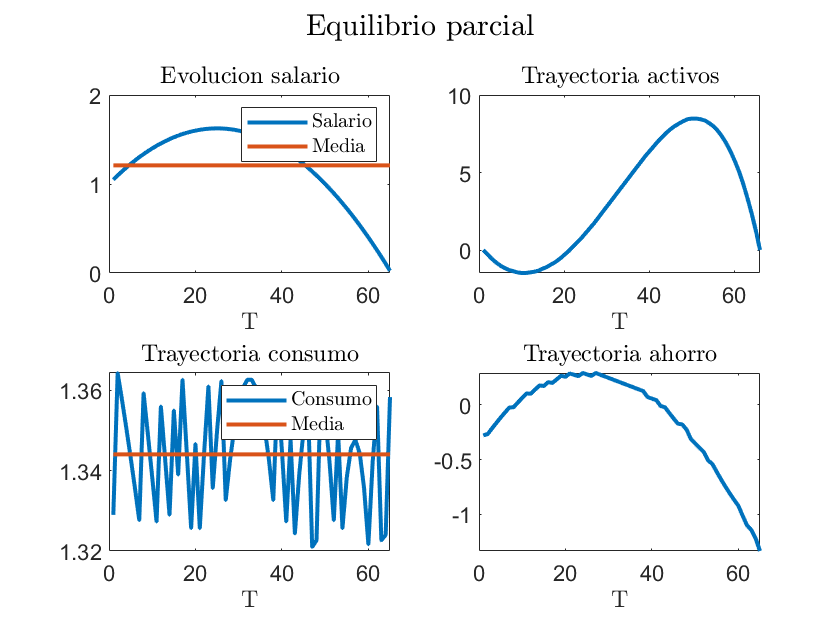
\includegraphics[width=\maxwidth{84.29503261414952em}]{image_0}
\end{flushleft}
\end{par}

\begin{par}
\begin{center}
Figura A. Trayectoria del ciclo de vida del agente
\end{center}
\end{par}


\vspace{1em}
\begin{par}
\begin{flushleft}
A partir de la Figura A podemos decir que respecto a la trayectoria de consumo podemos notar que pese a las variaciones de un periodo a otro, no es monótona ni creciente ni decreciente. Más bien, la sustitución intertemporal de un periodo a otro es bastante similarsi en t=0 el agente consumía menos del promedio, en el siguiente periodo consumía más que el promedio, pero en el subisguiente nuevamente consumía menos. Lo que si se puede destacar es que esos vaivenes en los niveles de consumo van disminuyendo sus rangos y permanencia a medida que el agente vive más periodos. Económicamente tiene sentido: al inicio podemos notar que entre 0 y 20 se dan periodos más grandes de consumo por sobre la media, lo que se puede deber a que durante estos periodos el agente tiene más ingreso salarial posible. Como podemos ver en la trayectoria de activos, al inicio debe endeudarse un poco para consumir (hasta el periodo 10). Esto ciertamente se corresponde con los resultados de la teoría de la renta permanente, donde el agente define su consumo bajo un horizonte finito, evaluando el valor esperado de sus ingresos. Solo en una pequeña parte del inicio de este tramo, el valor esperado del ingreso (línea naranja de figura sobre evolución salarial) es más alta que la función que muesta la distribución de los salarios. 
\end{flushleft}
\end{par}

\begin{par}
\begin{flushleft}
Además, tal como mostró Carrol (2001) en un contexto con mercado financiero perfecto, preferencias CRRA podemos observar que el motivo de ahorro de los jóvenes (hasta cerca del periodo 25) existe una restricción crediticia autoimpuesta donde el agente ahorra para poder suavizar consumo en los periodos que vienen ante la existencia de un ingreso salarial cero o muy bajo (como ocurre cerca ya del periodo 70). Reforzaremos este argumento viendo la policy function del consumo, capital y value function. 
\end{flushleft}
\end{par}

\begin{par}
\begin{flushleft}
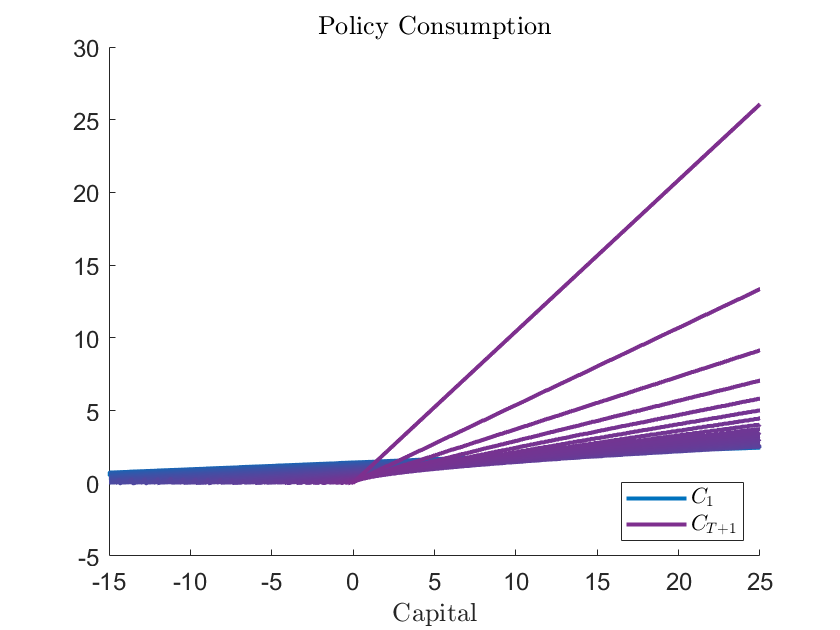
\includegraphics[width=\maxwidth{45.760160561966885em}]{image_1}
\end{flushleft}
\end{par}

\begin{par}
\begin{flushleft}
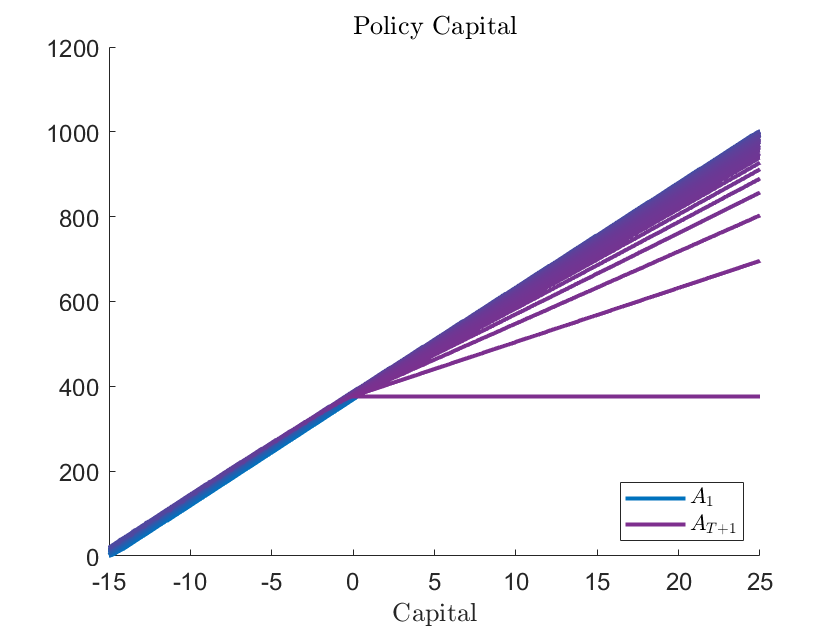
\includegraphics[width=\maxwidth{46.96437531359759em}]{image_2}
\end{flushleft}
\end{par}

\begin{par}
\begin{flushleft}
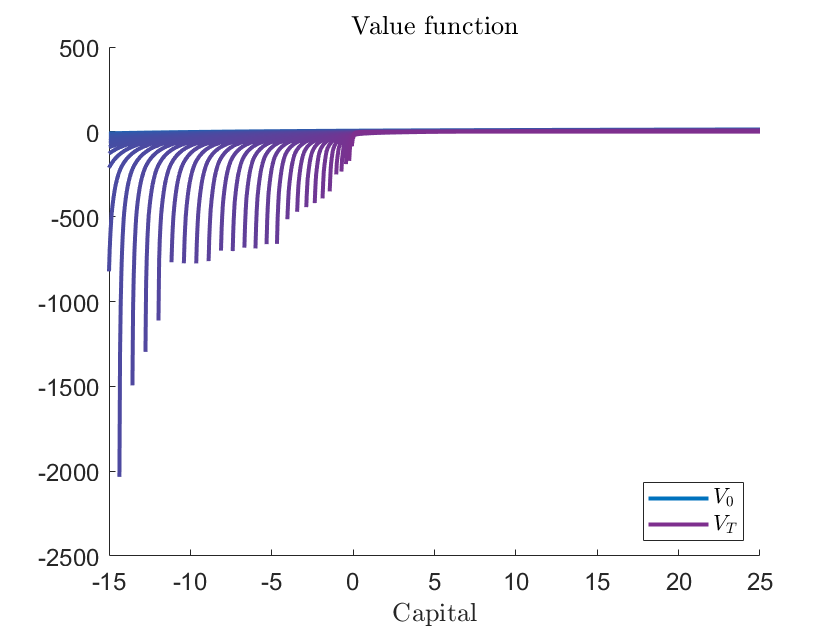
\includegraphics[width=\maxwidth{48.06823883592574em}]{image_3}
\end{flushleft}
\end{par}

\begin{par}
\begin{center}
Figura B. Policy y value function del problema del agente
\end{center}
\end{par}

\begin{par}
\begin{flushleft}
Primero, la figura de la policy function del consumo muestra como, sujeto a la restricción de no negatividad del consumo y las zonas factibles para el consumo, desde el periodo 0 se evidencia la decisión óptima del agente respecto a los activos dispoibles. A medida que más aumente el horizonte del agente, el agente suaviza mucho más su consumo. 
\end{flushleft}
\end{par}

\matlabheading{d. Cambio en el nivel inicial de los salarios}

\begin{par}
\begin{flushleft}
La evolución salarial no depende solo de la concavidad de la función, esto es a qué velocidad crece y luego decrecen los salarios, sino que también del nivel inicial de los salarios que tienen los agentes, lo que puede ser muy relevante para decidir la trayectoria de consumo y cuanto ahorrar o endeudarse para el consumo futuro. La razón: la edad en que los ingresos empiezan a bajar es distinta, junto con que el nivel de ingresos esperados al inicio puede dar más holgura para la liquidez si es que el nivel es mayor. Retomaremos este punto en el último problema de este informe, donde los salarios serán endógenos y la oferta laboral elástica. 
\end{flushleft}
\end{par}

\begin{par}
\begin{flushleft}
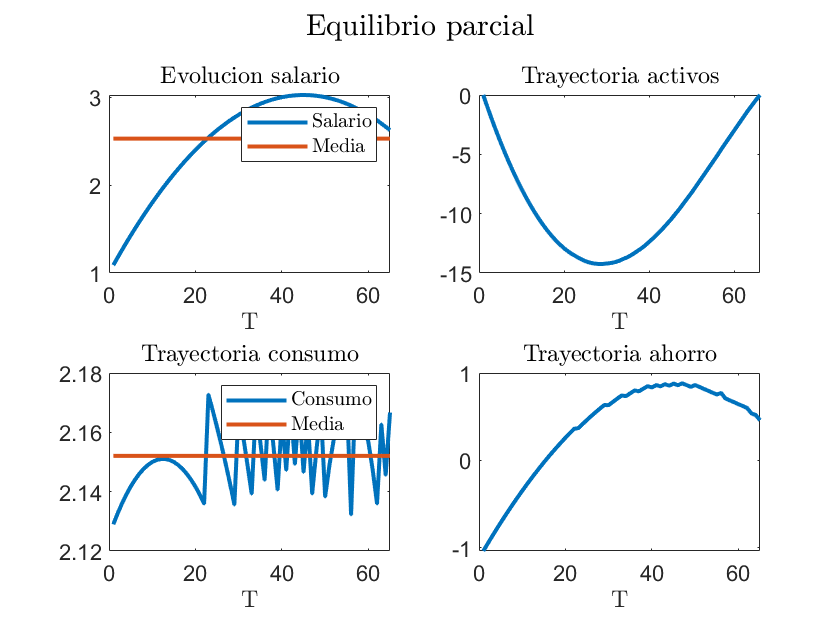
\includegraphics[width=\maxwidth{66.93426994480683em}]{image_4}
\end{flushleft}
\end{par}

\begin{par}
\begin{center}
Figura C. Trayectoria de ciclo de vida del agente con trayectoria salarial $w_2$
\end{center}
\end{par}

\begin{par}
\begin{flushleft}
Volviendo al punto inicial, gráficamente se ve en el siguiente figura donde la función que define la trayectoria laboral es $\;w_2 =\frac{-t^2 }{{10}^3 }+\frac{t}{{10}^2 }\cdot 9+1$ en donde $\frac{\partial }{\partial t}\left(-\frac{t^2 }{1000}+\frac{9t}{100}+1\right)=\frac{45-t}{500}\to t^* =45\;$, es decir, desde el periodo 45 de su ciclo de vida el retorno de la productividad marginal del trabajo empieza a ser decreciente y su nivel máximo alcanzado es de 3,025. A su vez, el agente parte con un salario de 1 al inicio de su ciclo y muere con un salario de 2,4 en el periodo 70. 
\end{flushleft}
\end{par}

\begin{par}
\begin{flushleft}
En contraste, para la trayectoria laboral $\;w_1 =\;\frac{-t^2 }{{10}^3 }+\frac{t}{{10}^2 }\cdot 5+1$ en donde$\frac{\partial }{\partial t}\left(-\frac{t^2 }{1000}+\frac{t}{20}+1\right)=\frac{25-t}{500}\to t^* =25\;$, es decir, desde el periodo 25 del ciclo de vida del agente el retorno de la productividad marginal del trabajo empieza a ser decreciente y su nivel máximo alcanzado es cercano a 1.5 . Al igual que antes, el agente parte con un salario de 1 al inicio de su ciclo y pero cerca del periodo 70 ya no recibe ingresos. 
\end{flushleft}
\end{par}

\begin{par}
\begin{flushleft}
Como podemos notar, la tendencia de consumo, en general no varía mucho en su forma, solo que particularmente al inicio del ciclo de vida el agente va a consumir un poco menos (hasta periodo 15) pero no totalmente dado que va a recurrir a deuda para poder alcanzar su nivel de consumo.
\end{flushleft}
\end{par}

\begin{par}
\begin{flushleft}
Recordemos que de la versión moderna de la teoría de la renta permanente, los agentes deciden su consumo sujeto al valor esperado de sus ingresos (pensemos salariales) y que su ahorro está sujeto a shocks de ingreso. En este caso, la primera parte del ciclo de vida evidentemente el agente está bajo el valor esperado del ingreso, por lo que su consumo será levemente más bajo.  Los jovenes que ahorrán de manera autoimpuesta y hacia el final del ciclo los agentes tendrán un ingreso mayor que en los inicios de la vida laboral. De hecho, el ahorro de los agentes desde el punto de inflexión del periodo 45 comienzan a disminuir su ahorro y consumir todo lo que que tienen guardado.
\end{flushleft}
\end{par}

\matlabheading{e. Transformaciones afines en los salarios y cambio de parámetros sobre el trade off del consumo en t y t+1}

\begin{par}
\begin{flushleft}
Ahora nuevamente cambiaremos la trayectoria del salario a $w_3 =-{10}^{-2} t^2 +7\cdot {10}^{-2} t+1$ y la tasa de interés a $r=0\ldotp 05$ y la aversión al riesgo a $\sigma =8$. Para hacer comparables los resultados, hemos resuelto el problema del agente con sus múltiples combinaciones, para ver afectivamente cuál es el peso del factor psicológico, económico y la aversión al riesgo sobre la decisión del agente. La representación gráfica de esto está en la Figura D
\end{flushleft}
\end{par}

\begin{par}
\begin{flushleft}
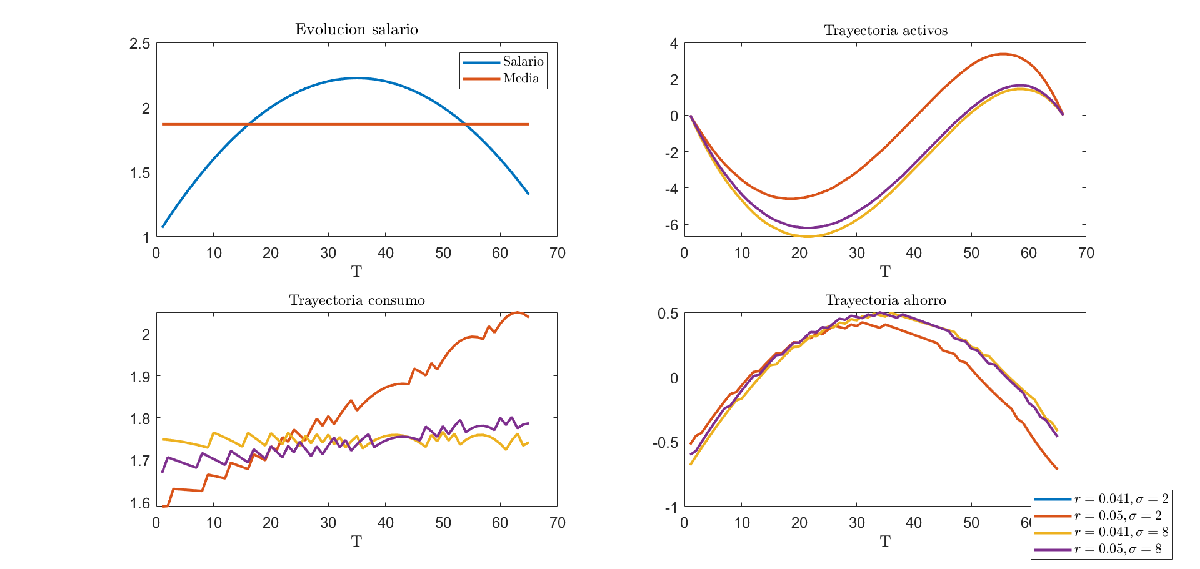
\includegraphics[width=\maxwidth{101.9568489713999em}]{image_5}
\end{flushleft}
\end{par}

\begin{par}
\begin{center}
Figura D. Trayectorias del agente a un nivel salarial $w_3$
\end{center}
\end{par}

\begin{par}
\begin{flushleft}
Respecto a la Figura D podemos notar que se reportan, para un nivel de salarios dado, tres trayectorias de consumo, ahorro y activos (curva naranja, amarilla y morada). La trayectoria azul no aparece pues, como se puede verificar en su resolucion numerica (figuremultiple.m línea 15 y 17) sus valores son iguales. Comentaremos esto más adelante, dada las implicancias de una tasa  $r=\frac{1-\beta }{\beta }$. Ahora bien, partamos analizando parte por parte la figura:
\end{flushleft}
\end{par}

\begin{enumerate}
\setlength{\itemsep}{-1ex}
   \item{\begin{flushleft} La trayectoria del consumo muestra que, tanto la trayectoria de consumo con tasa 0.041 y 0.05 suavizan consumo, con una aversión al riesgo alta. En ese sentido, controlando por el salario, notaremos que las trayectorias con menor tasa de interés pero con agentes más aversos al riesgo, se producirá que los agentes consumirán en cantidades similares hoy y mañana. Mientras que en el caso de la trayectoria naranja, notaremos que el agente valora mucho más los retornos en el futuro dado que la tasa de interés es más alta y su aversión al riesgo es mucho más baja, por lo que el agente preferirá consumir menos hoy para asegurar consumo futuro. En ese sentido, podremos notar que $r>\rho$ ($\rho$ es tasa de descuento), por lo que el agente pondera mucho más el factor económico que el psicológico en su decisión (incertidumbre e impaciencia).  \end{flushleft}}
   \item{\begin{flushleft} La trayectoria de activos es coherente con lo que hemos indicado. Notemos que a diferencia de la curva púrpura y amarilla, la trayectoria naranja se endeuda mucho menos en la primera parte de su vida, pues prefiere ahorrar para consumir más en el futuro. Pensemos, además, que la tasa de interés es el precio de los activos, por lo que a ese nivel el precio del activo es mayor que en el caso de la curva amarilla. ¿Pero qué pasa con la curva púrpura? Este agente es más averso al riesgo que el naranja, por lo que inclusive considerando el precio del capital, prefiere consumir igual hoy que mañana. Por lo mismo, su nivel de endeudamiento será mayor en su primera etapa de vida, comparado con el agente naranja. \end{flushleft}}
   \item{\begin{flushleft} Ahora bien, la trayectoria del ahorro es bastante similar. Solo en el caso del agente naranja es un poco superior en la primera parte del ciclo de vida e inferior en la segunda parte. Probablemente la razón de esa similitud se deba a que si bien al inicio el agente naranja consume menos que el agente amarillo, púrpura y azul (lo que lleva a ahorrar más al naranja), los otros agentes ahorren de igual forma por un motivo precautorio.  \end{flushleft}}
\end{enumerate}

\begin{par}
\begin{flushleft}
Una pregunta que surge evidentemente de este análisis es, ¿qué implicancias tiene $r=\frac{1-\beta }{\beta }$ sobre trayectoria de activos óptima (y sobre el ahorro)?  Notamos que la curva azul y la amarrila son iguales, es decir, independiente de la aversión al riesgo los agentes tienen la misma trayectoria. Partiremos primero resolviendo la tasa de interés, y luego discutiremos sus implicancias económicas. 
\end{flushleft}
\end{par}

\begin{par}
\begin{flushleft}
La derivación de $r=\frac{1-\beta }{\beta }$ parte de suponer que tenemos a un agente indiferente entre la utilidad del consumo que da $u\left(c_t \right)\;y\;u\left(c_{t+1} \right)$, esto implica que los dos factores que determinan la trayectoria de consumo del agente, esto es, el factor psicológico $\beta \;\left(\textrm{impaciencia}\right)$ y el económico $R\;\left(\textrm{precio}\;\textrm{de}\;\textrm{los}\;\textrm{activos}\right)$, se netean ($\beta R=1$.) Nosotros además sabemos que $\beta =\frac{1}{1+\rho }$, donde $\rho$ es la tasa de descuento y $R=\left(1+r\right)$ donde r es la tasa de interés real. Si reemplazamos estas dos cosas obtenemos
\end{flushleft}
\end{par}

\begin{par}
$$\frac{1}{1+\rho }\cdot \left(1+r\right)=1\leftrightarrow \frac{1}{1+\rho }=\frac{1}{1+r}$$
\end{par}

\begin{par}
\begin{flushleft}
Entonces cuando $\beta R=1$ entonces $\rho =r$ , en ese caso $c_1 =c_2$. En este caso no hay incentivo de ahorro ni de consumo.
\end{flushleft}
\end{par}

\begin{par}
$$1+r=\frac{1}{\beta }\;\leftrightarrow r=\frac{1}{\beta }-1\leftrightarrow r=\frac{1-\beta }{\beta }$$
\end{par}

\begin{par}
\begin{flushleft}
Volviendo a la gráfica notaremos que entonces, tanto el factor económico como el psicológico son igualmente ponderados por el agente. Así, a ese nivel de tasa de interés, independiente de si el agente es más o menos averso al riesfo este será indiferente entre consumir hoy o consumir mañana. Esto no significa que los agentes entonces decidan consumir todo hoy o todo mañana. No. Solo estamos diciendo que no existe una preferencia por un periodo u otro, pero este agente sigue teniendo por objetivo suavizar consumo  (por ello la trayectoria plana entre cada t y t+1) y sigue siendo prudente (y por ello no deja de ahorrar). 
\end{flushleft}
\end{par}

\end{document}
